

%%% This LaTeX source document can be used as the basis for your technical
%%% report. Intentionally stripped and simplified
%%% and commands should be adjusted for your particular paper - title, 
%%% author, citations, equations, etc.
% % Citations/references are in report.bib 

\documentclass[conference,backref=page]{acmsiggraph}

\TOGonlineid{45678}
\TOGvolume{0}
\TOGnumber{0}
\TOGarticleDOI{1111111.2222222}
\TOGprojectURL{}
\TOGvideoURL{}
\TOGdataURL{}
\TOGcodeURL{}

\usepackage{listings}


% Include this so that citations show up in blue and the page information is included in the reference section
\hypersetup{
    colorlinks = true, 
    linkcolor = blue,
    anchorcolor = red,
    citecolor = blue, 
    filecolor = red, 
}

%Macro for figures
\newcommand{\figuremacro}[5]{
	\begin{figure}[#1]
		\centering
		\includegraphics[width=#5\columnwidth]{images/#2}
		\caption[#3]{\textbf{#3}#4}
		\label{fig:#2}
	\end{figure}
}

%code layout
\lstset{
	escapeinside={/*@}{@*/}, language=C++,
	basicstyle=\fontsize{8.5}{12}\selectfont,
	numbers=left,numbersep=2pt,xleftmargin=2pt,frame=tb,
	columns=fullflexible,showstringspaces=false,tabsize=4,
	keepspaces=true,showtabs=false,showspaces=false,
	backgroundcolor=\color{white}, morekeywords={inline,public,
		class,private,protected,struct},captionpos=t,lineskip=-0.4em,
	aboveskip=10pt, extendedchars=true, breaklines=true,
	prebreak = \raisebox{0ex}[0ex][0ex]{\ensuremath{\hookleftarrow}},
	keywordstyle=\color[rgb]{0,0,1},
	commentstyle=\color[rgb]{0.133,0.545,0.133},
	stringstyle=\color[rgb]{0.627,0.126,0.941}
}


\title{Physics Simulation Evaluation}

\author{Zoe Wall
 \thanks{40182161@live.napier.ac.uk} \\
Edinburgh Napier University\\
Physics-Based Animation (SET09119)}
\pdfauthor{Zoe Wall}

\keywords{resonance, openGL, real-time rendering, physics, Chlandi, standing waves, fundamental frequencies, cloth, mass-spring systems}

\begin{document}

\teaser{
	\centering
   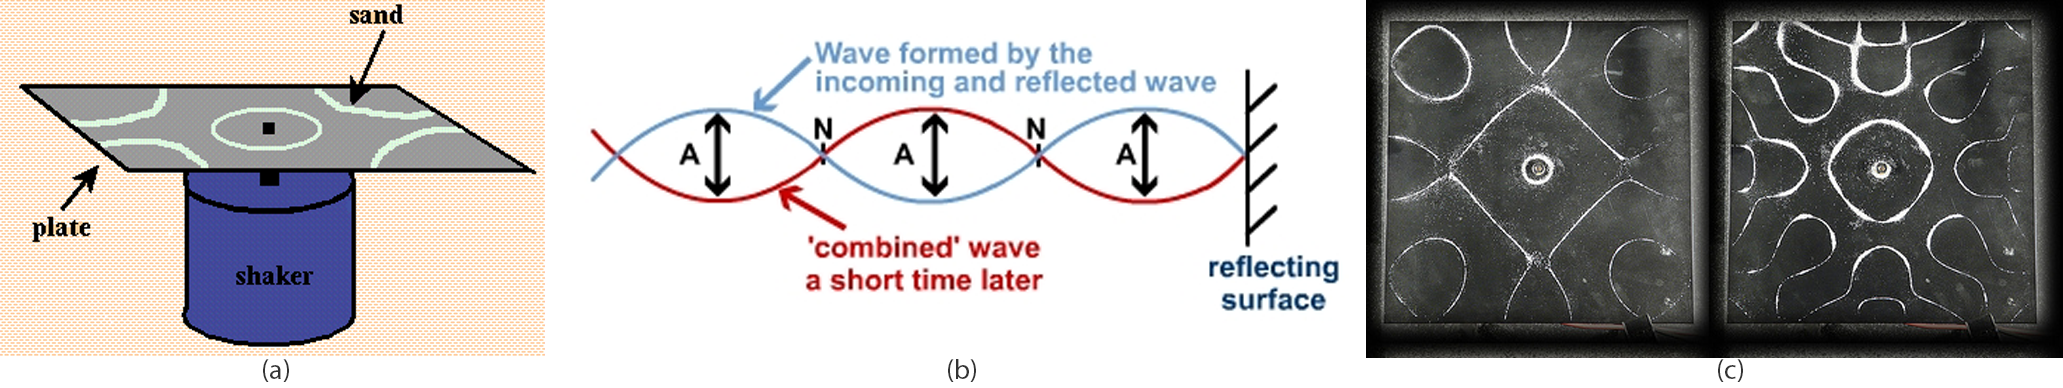
\includegraphics[width=\textwidth,height=1.5in]{images/teaser}
   \caption{(a) diagram of Chlandi plate experiment, (b) diagram to show standing waves, and (c) an image of salt patterns showing the different modes. }
   \label{fig:teaser}
 }

\maketitle

\raggedbottom

\begin{abstract}
This paper presents the implementation methods made in an attempt to render a realistic physics simulation of a Chlandi plate experiment in real-time. The visualisation consists of a square grid, similar to that of a trampoline, with particles bouncing ontop of it. This is interactive through the use of a graphical user interface which allows the user to add or remove particles. The simulation was implemented in c++ with OpenGL. 	

\end{abstract}



\keywordlist

%% Use this only if you're preparing a technical paper to be published in the 
%% ACM 'Transactions on Graphics' journal.

% \TOGlinkslist

% \copyrightspace


\section{Introduction}

The goal of this project was to create a physics-based simulation of a Chlandi plate. A Chlandi plate is an example of an experiment into resonance, by studying the motion of a vibrating membrane. The experiment consists of sprinkling sand onto the surface of a metal plate and exciting the plate at a certain frequency. This was a very early way to visualise the effects of vibrations through a surface as at certain discrete frequencies patterns would form in the sand. These patterns are formed by standing waves propagating throughout the metal, at the areas of no displacement the sand settles.

Unfortunately, driving the simulation in such a way that the mass-spring system resonated proved to be extremely difficult. Waves can be seen to propagate within the mesh, see figure \ref{fig:wave}, however something so consistent as a standing wave was not accomplished. 

\figuremacro{h}{wave}{Screenshot of simulation}{ - still frame showing the mesh displacement.}{1.0}

This was one of the major limitations outlined within the project plan, due to the fact that the in the real world, when systems are driven, it is hard for them to vibrate at a frequency that isn't the systems natural frequency or a harmonic of it. The mass spring system, another challenge to the project was successfully implemented along with the particle collision detection. 

\section{Related Work}

Drawing inspiration from the Mass Spring Damper Model - a technique used in real-time cloth rendering. The main challenge of this project is to design and implement a model of a metal plate that is able to vibrate. The Mass Spring Damper Model for cloth simulation is based of a grid of particles connected together by spring-dampers. There are three different types of forces exerted by the spring-dampers depending on how they connect particles, see figure \ref{fig:cloth}. Structural springs handle horizontal and vertical constraints such as extension or depression; shear springs handle stresses that are parallel to the material and are connected diagonally; whilst bend springs are connected horizontally and vertically but between every other particle. \cite{clothism}

\figuremacro{h}{cloth}{Cloth Forces}{ - diagram to show the three different types of forces that can be exerted by a spring-damper: structural, shear and bending.\cite{clothforce}}{1.0}

\section{Overview}
The core computer graphics principles which were goals of the implementation are as follows:
\begin{itemize}
	\item Mass Spring Systems
	\item Particle Effects
	\item Collision Detection
\end{itemize}

Although the overall effect was not as planned, the simulation covered each of these principles to a good degree. The mass spring system is the basis of the simulation, created with a mesh of interconnected points that apply forces to each other, according to Hooke's law. Detection of collisions between this mesh and any particles dropped on it, was implemented using sphere-to-sphere intersection tests and the collisions were resolved resulting in a trampoline-like simulation. 

\section{Simulation}

%SCREENSHOT HERE

\subparagraph{Functionality}

As described within the design document, the simulation should have been a real-time demonstration of standing waves forming within a surface, of which displaces particles dropped from above. However the final result of the functionality of the simulation did not produce standing waves and therefore a driving force at a frequency was not implemented, so the interactivity was changed. The user instead can give an impulse to a section of the grid, insert or remove particles to be dropped on the plate and as outlined in the plan, freely move the camera using the WASD keys.

\subparagraph{Method}
 The visual effect of waves propagating throughout the surface is implemented using simple harmonic motion.

Simple harmonic motion is defined as the behaviour of a mass-spring damper where the forces acting on the mass given by Hooke's Law: equation \ref{eq:hooke} below:

 \begin{equation} \label{eq:hooke}
 F = -kx
 \end{equation}

 where F is the force to stretch the spring, k is the spring constant - how stiff the spring is, and x is the displacement of the spring.
 
 This forms the basis of the simulation as it must show a wave propagating within the plate, see figure \ref{fig:eigen}. After the metal is moving, the particles on the surface should be displaced by the movement, and settle within the areas of no displacement from the waves.
 
 This relies on particle collision detection.
 
 \figuremacro{h}{eigen}{Diagrams of different modes}{- there are certain discrete frequencies that will cause the plate to vibrate in different ways. \cite{modes}}{1.0}
 
 The collision detection will be implemented through the use of bounding spheres for the particles and possibly for each node within the plate mesh. This is something that needs to be tested, to determine which is the best boundaries to set for the plate.

\subparagraph{Interactivity}The simulation will be controlled through a user interface, the user should be able to pick certain frequencies for the plate-driver from a sliding scale. The camera will also be controlled through keyboard and mouse movement. To stop the mouse movement interfering with the view of the camera when the user is trying to select items within the UI, the right mouse button held down will be used to drag the camera view around. There will also be an option in the UI so the user can switch to view a static camera.

\section{Implementation}

It is anticipated that one of the major software development tasks will be in the implementation of the surface. At this stage in the project it is unclear that the simple harmonic motion will be visible. This is a major project risk with implementation due to the fact that the time-step could be too high to achieve the frequency of the driver or the resolution of the plate. If it becomes unachievable, the project will still model a cloth-system with particle collision detection, however the frequency driver will not be present. Instead the project can be more akin to a trampoline simulation. With the plate becoming a stiff cloth still constrained by its edges, and the particles will be 'bounced' by the user.

An external library called ImGui \cite{imgui} will be used to implement a graphical user interface for debugging and frame-rate monitoring. ImGui is a third-party open source library which will allow for custom buttons and sliders to be overlaid over the simulation for the user to interact with.


%STARTS

To run a smooth real-time simulation the physics must be updated once per tick, not per frame. Therefore per frame, the update function has to calculate the ticks, and perform the physics update. A fixed time step method was used, see code listing \ref{lst:tick}.

\begin{lstlisting}[caption = {update function called per frame}, label = {lst:tick}]
	static double t = 0.0;
	static double accumulator = 0.0;
	accumulator += delta_time;
	
	while (accumulator > physics_tick)
	{
		// update physics each tick
		myMan.update_physics(t, physics_tick);
		accumulator -= physics_tick;
		t += physics_tick;
	}
\end{lstlisting}

This means that if there is not enough time to complete a full tick, the remaining time is added to the next frame and an extra tick could be carried out then. A tick only occurs once a fixed time has passed, in this case physics\_tick was defined as 1/60th.

\subsection{Update Physics Loop}

Every tick, the update physics function would be called. This executes first the collision detection,
col resolution
spring update
integrate springs
integrate balls


In order to simulate the vertex displacement of the metal plate in the experiment, a different approach to constructing the rendered object was needed, as each vertex could move meaning the geometry had to be dynamic.
To render a series of points in OpenGL.


\paragraph{Plate} - In constructing the plate, a two-dimensional array of Atom objects was used for storing information.


 implemented a mass-spring system.

\section{Testing and evaluation}

To make the testing easier the implementation the project will be split into separate goals. First, making the plate resonate. To test this, by using ImGui the frame-rate and time-step can be monitored as the application is running. A small low-resolution grid will be the starting point. Similarly with the particle collision detection, the starting point will be one particle, with the intention of adding more. Testing is quite challenging due to the nature of OpenGL, everything will have to be visual. To test to see if the physics is realistic will take trial and error as the physical values, for example the spring constant, are almost arbitrary.

\section{Conclusion}

In conclusion, this project will be very challenging to implement as it has many limitations with regards to performance and time. However, if achievable this simulation be used to demonstrate a real-world physical phenomenon. 


% \section*{Acknowledgements}

% SORT BIB OUT
\bibliographystyle{acmsiggraph}
\bibliography{report}

\end{document}

